\documentclass[conference]{IEEEtran}


% *** GRAPHICS RELATED PACKAGES ***
%
\ifCLASSINFOpdf
  \usepackage[pdftex]{graphicx}
  % declare the path(s) where your graphic files are
  % \graphicspath{{../pdf/}{../jpeg/}}
  % and their extensions so you won't have to specify these with
  % every instance of \includegraphics
  % \DeclareGraphicsExtensions{.pdf,.jpeg,.png}
\else
  % or other class option (dvipsone, dvipdf, if not using dvips). graphicx
  % will default to the driver specified in the system graphics.cfg if no
  % driver is specified.
  % \usepackage[dvips]{graphicx}
  % declare the path(s) where your graphic files are
  % \graphicspath{{../eps/}}
  % and their extensions so you won't have to specify these with
  % every instance of \includegraphics
  % \DeclareGraphicsExtensions{.eps}
\fi
% graphicx was written by David Carlisle and Sebastian Rahtz. It is
% required if you want graphics, photos, etc. graphicx.sty is already
% installed on most LaTeX systems. The latest version and documentation
% can be obtained at: 
% http://www.ctan.org/tex-archive/macros/latex/required/graphics/
% Another good source of documentation is "Using Imported Graphics in
% LaTeX2e" by Keith Reckdahl which can be found at:
% http://www.ctan.org/tex-archive/info/epslatex/
%
% latex, and pdflatex in dvi mode, support graphics in encapsulated
% postscript (.eps) format. pdflatex in pdf mode supports graphics
% in .pdf, .jpeg, .png and .mps (metapost) formats. Users should ensure
% that all non-photo figures use a vector format (.eps, .pdf, .mps) and
% not a bitmapped formats (.jpeg, .png). IEEE frowns on bitmapped formats
% which can result in "jaggedy"/blurry rendering of lines and letters as
% well as large increases in file sizes.
%
% You can find documentation about the pdfTeX application at:
% http://www.tug.org/applications/pdftex





% *** MATH PACKAGES ***
%
\usepackage[cmex10]{amsmath}
% A popular package from the American Mathematical Society that provides
% many useful and powerful commands for dealing with mathematics. If using
% it, be sure to load this package with the cmex10 option to ensure that
% only type 1 fonts will utilized at all point sizes. Without this option,
% it is possible that some math symbols, particularly those within
% footnotes, will be rendered in bitmap form which will result in a
% document that can not be IEEE Xplore compliant!
%
% Also, note that the amsmath package sets \interdisplaylinepenalty to 10000
% thus preventing page breaks from occurring within multiline equations. Use:
%\interdisplaylinepenalty=2500
% after loading amsmath to restore such page breaks as IEEEtran.cls normally
% does. amsmath.sty is already installed on most LaTeX systems. The latest
% version and documentation can be obtained at:
% http://www.ctan.org/tex-archive/macros/latex/required/amslatex/math/





% *** SPECIALIZED LIST PACKAGES ***
%
%\usepackage{algorithmic}
% algorithmic.sty was written by Peter Williams and Rogerio Brito.
% This package provides an algorithmic environment fo describing algorithms.
% You can use the algorithmic environment in-text or within a figure
% environment to provide for a floating algorithm. Do NOT use the algorithm
% floating environment provided by algorithm.sty (by the same authors) or
% algorithm2e.sty (by Christophe Fiorio) as IEEE does not use dedicated
% algorithm float types and packages that provide these will not provide
% correct IEEE style captions. The latest version and documentation of
% algorithmic.sty can be obtained at:
% http://www.ctan.org/tex-archive/macros/latex/contrib/algorithms/
% There is also a support site at:
% http://algorithms.berlios.de/index.html
% Also of interest may be the (relatively newer and more customizable)
% algorithmicx.sty package by Szasz Janos:
% http://www.ctan.org/tex-archive/macros/latex/contrib/algorithmicx/




% *** ALIGNMENT PACKAGES ***
%
%\usepackage{array}
% Frank Mittelbach's and David Carlisle's array.sty patches and improves
% the standard LaTeX2e array and tabular environments to provide better
% appearance and additional user controls. As the default LaTeX2e table
% generation code is lacking to the point of almost being broken with
% respect to the quality of the end results, all users are strongly
% advised to use an enhanced (at the very least that provided by array.sty)
% set of table tools. array.sty is already installed on most systems. The
% latest version and documentation can be obtained at:
% http://www.ctan.org/tex-archive/macros/latex/required/tools/


% IEEEtran contains the IEEEeqnarray family of commands that can be used to
% generate multiline equations as well as matrices, tables, etc., of high
% quality.




% *** SUBFIGURE PACKAGES ***
%\ifCLASSOPTIONcompsoc
%  \usepackage[caption=false,font=normalsize,labelfont=sf,textfont=sf]{subfig}
%\else
%  \usepackage[caption=false,font=footnotesize]{subfig}
%\fi
% subfig.sty, written by Steven Douglas Cochran, is the modern replacement
% for subfigure.sty, the latter of which is no longer maintained and is
% incompatible with some LaTeX packages including fixltx2e. However,
% subfig.sty requires and automatically loads Axel Sommerfeldt's caption.sty
% which will override IEEEtran.cls' handling of captions and this will result
% in non-IEEE style figure/table captions. To prevent this problem, be sure
% and invoke subfig.sty's "caption=false" package option (available since
% subfig.sty version 1.3, 2005/06/28) as this is will preserve IEEEtran.cls
% handling of captions.
% Note that the Computer Society format requires a larger sans serif font
% than the serif footnote size font used in traditional IEEE formatting
% and thus the need to invoke different subfig.sty package options depending
% on whether compsoc mode has been enabled.
%
% The latest version and documentation of subfig.sty can be obtained at:
% http://www.ctan.org/tex-archive/macros/latex/contrib/subfig/




% *** FLOAT PACKAGES ***
%
%\usepackage{fixltx2e}
% fixltx2e, the successor to the earlier fix2col.sty, was written by
% Frank Mittelbach and David Carlisle. This package corrects a few problems
% in the LaTeX2e kernel, the most notable of which is that in current
% LaTeX2e releases, the ordering of single and double column floats is not
% guaranteed to be preserved. Thus, an unpatched LaTeX2e can allow a
% single column figure to be placed prior to an earlier double column
% figure. The latest version and documentation can be found at:
% http://www.ctan.org/tex-archive/macros/latex/base/


%\usepackage{stfloats}
% stfloats.sty was written by Sigitas Tolusis. This package gives LaTeX2e
% the ability to do double column floats at the bottom of the page as well
% as the top. (e.g., "\begin{figure*}[!b]" is not normally possible in
% LaTeX2e). It also provides a command:
%\fnbelowfloat
% to enable the placement of footnotes below bottom floats (the standard
% LaTeX2e kernel puts them above bottom floats). This is an invasive package
% which rewrites many portions of the LaTeX2e float routines. It may not work
% with other packages that modify the LaTeX2e float routines. The latest
% version and documentation can be obtained at:
% http://www.ctan.org/tex-archive/macros/latex/contrib/sttools/
% Do not use the stfloats baselinefloat ability as IEEE does not allow
% \baselineskip to stretch. Authors submitting work to the IEEE should note
% that IEEE rarely uses double column equations and that authors should try
% to avoid such use. Do not be tempted to use the cuted.sty or midfloat.sty
% packages (also by Sigitas Tolusis) as IEEE does not format its papers in
% such ways.
% Do not attempt to use stfloats with fixltx2e as they are incompatible.
% Instead, use Morten Hogholm'a dblfloatfix which combines the features
% of both fixltx2e and stfloats:
%
% \usepackage{dblfloatfix}
% The latest version can be found at:
% http://www.ctan.org/tex-archive/macros/latex/contrib/dblfloatfix/




% *** PDF, URL AND HYPERLINK PACKAGES ***
%
%\usepackage{url}
% url.sty was written by Donald Arseneau. It provides better support for
% handling and breaking URLs. url.sty is already installed on most LaTeX
% systems. The latest version and documentation can be obtained at:
% http://www.ctan.org/tex-archive/macros/latex/contrib/url/
% Basically, \url{my_url_here}.



% correct bad hyphenation here
\hyphenation{op-tical net-works semi-conduc-tor}

\providecommand{\keywords}[1]{\textbf{\textit{Index Terns---}} #1}


\begin{document}
\title{An Acoustic Recognition End-to-end System on Under-resources Languages}

\author{

\IEEEauthorblockN{Chun-Hao Wang}
\IEEEauthorblockA{Department of Computer Science \\
National Taiwan University\\
chuchuhao831@gmail.com }
\and
\IEEEauthorblockN{Kuan-Hou Chan}
\IEEEauthorblockA{Department of Computer Science \\
National Taiwan University\\
iepiechan@gmail.com  }
}

% make the title area
\maketitle

\begin{abstract}
With the rapid development of sequence learning techniques, the state-of-the-art speech recognition system have a great performance on English speech corpus with almost human ability.  Compare to others under-resourced language which is less language-specific knowledge or less hand-labeling data is still an active field for research and still have no good performance.  Instead to find a system can make a good performance on some language recognize problem, we present a end-to-end system that directly translate the acoustic sequence to label sequence without any language-specific knowledge so that we can adapt on any language without much resources.  An experiment on the Cebuano speech corpus demonstrates its ability indeed learning some pattern from data.\\
\end{abstract}

\keywords{under-resources language, minority languages, connectionist temporal classification (CTC), sequence learning, speech and language resources, automatic speech recognition (ASR), cross-lingual acoustic modeling.}


% For peer review papers, you can put extra information on the cover
% page as needed:
% \ifCLASSOPTIONpeerreview
% \begin{center} \bfseries EDICS Category: 3-BBND \end{center}
% \fi
%
% For peerreview papers, this IEEEtran command inserts a page break and
% creates the second title. It will be ignored for other modes.
\IEEEpeerreviewmaketitle



\section{Introduction}
Speech recognition problem takes advantage of recent advance in algorithms and computer hardware, using the artificial neural networks (ANNs) techniques acquire a good performance on the task.  According to the Grave's research[2],{\it a end-to-end system achieves a word error rate of 27.3\% on the Wall Street Journal corpus with no prior linguistic information, 21.9\% with only a lexicon of allowed words, and 8.2\% with a trigram language model. Combining the network with a baseline system further reduces the error rate to 6.7\%}.  Not only to this end-to-end system acquire that perfect result, there also some graphical models such as hidden Markov Models (HMMs; Rabiner), conditional random field (CRFs; Lafferty) hybrid with ANNs and the aggregation of different models with additional language-specific feature, all of them do the great job.  While all of these approaches performed excellent, but they usually have to use lots of language resources which from large hand-labeling acoustic sequence to label sequence pair to some knowledge like phoneme and feature theory except the Grave's RNN-CTC system.  Grave's system can achieves low error rate in English corpus without prior linguistic information, and we assume such characteristic which regardless of linguistic information let us be able to apply the system on some other language. \\
So far, the speech recognition problem on under-resourced language is still an active field for research, and we expect that if we could apply a system without the language-specific knowledge (like the Grammer, Grapheme and Phonology) and less labeling data then we create a system as the speech-to-text machine on all the language in the world. We believe we can break the language barrier for human communication.  \\
To define clarity, we seem this as a sequence learning problem which labeling unsegmented sequence data or to say unsupervised learning the temporal classification[4]. Input a time various speech sequence data and output a sequence of label, for example, we take the filter-bank extract acoustic features from the speech signal with a fixed frame size as input  and turn them into a sequence of labels which is English Character as output.  \\
In our experiment we use bidirectional long short-term memory as our neural unit with their powerful, general mechanism for modelling time series and connectionist temporal result (CTC) output to let the RNN-alone sequence learning become possible.  \\
The next section introduce bidirectional long short-term memory (BLSTM) and connectionist temporal classification (CTC) and briefly describe how them be trained, output representation and build our recognition system.  Section 3 describe the Cebuano speech corpus we use in our experiment.  Section 4 present our experiment result and discuss them.  Section 5 makes a conclusion and provide list of further work we are on the process to solve this problem. 

% An example of a floating figure using the graphicx package.
% Note that \label must occur AFTER (or within) \caption.
% For figures, \caption should occur after the \includegraphics.
% Note that IEEEtran v1.7 and later has special internal code that
% is designed to preserve the operation of \label within \caption
% even when the captionsoff option is in effect. However, because
% of issues like this, it may be the safest practice to put all your
% \label just after \caption rather than within \caption{}.
%
% Reminder: the "draftcls" or "draftclsnofoot", not "draft", class
% option should be used if it is desired that the figures are to be
% displayed while in draft mode.
%
%\begin{figure}[!t]
%\centering
%\includegraphics[width=2.5in]{myfigure}
% where an .eps filename suffix will be assumed under latex, 
% and a .pdf suffix will be assumed for pdflatex; or what has been declared
% via \DeclareGraphicsExtensions.
%\caption{Simulation results for the network.}
%\label{fig_sim}
%\end{figure}

% Note that IEEE typically puts floats only at the top, even when this
% results in a large percentage of a column being occupied by floats.


% An example of a double column floating figure using two subfigures.
% (The subfig.sty package must be loaded for this to work.)
% The subfigure \label commands are set within each subfloat command,
% and the \label for the overall figure must come after \caption.
% \hfil is used as a separator to get equal spacing.
% Watch out that the combined width of all the subfigures on a 
% line do not exceed the text width or a line break will occur.
%
%\begin{figure*}[!t]
%\centering
%\subfloat[Case I]{\includegraphics[width=2.5in]{box}%
%\label{fig_first_case}}
%\hfil
%\subfloat[Case II]{\includegraphics[width=2.5in]{box}%
%\label{fig_second_case}}
%\caption{Simulation results for the network.}
%\label{fig_sim}
%\end{figure*}
%
% Note that often IEEE papers with subfigures do not employ subfigure
% captions (using the optional argument to \subfloat[]), but instead will
% reference/describe all of them (a), (b), etc., within the main caption.
% Be aware that for subfig.sty to generate the (a), (b), etc., subfigure
% labels, the optional argument to \subfloat must be present. If a
% subcaption is not desired, just leave its contents blank,
% e.g., \subfloat[].


% An example of a floating table. Note that, for IEEE style tables, the
% \caption command should come BEFORE the table and, given that table
% captions serve much like titles, are usually capitalized except for words
% such as a, an, and, as, at, but, by, for, in, nor, of, on, or, the, to
% and up, which are usually not capitalized unless they are the first or
% last word of the caption. Table text will default to \footnotesize as
% IEEE normally uses this smaller font for tables.
% The \label must come after \caption as always.
%
%\begin{table}[!t]
%% increase table row spacing, adjust to taste
%\renewcommand{\arraystretch}{1.3}
% if using array.sty, it might be a good idea to tweak the value of
% \extrarowheight as needed to properly center the text within the cells
%\caption{An Example of a Table}
%\label{table_example}
%\centering
%% Some packages, such as MDW tools, offer better commands for making tables
%% than the plain LaTeX2e tabular which is used here.
%\begin{tabular}{|c||c|}
%\hline
%One & Two\\
%\hline
%Three & Four\\
%\hline
%\end{tabular}
%\end{table}


% Note that the IEEE does not put floats in the very first column
% - or typically anywhere on the first page for that matter. Also,
% in-text middle ("here") positioning is typically not used, but it
% is allowed and encouraged for Computer Society conferences (but
% not Computer Society journals). Most IEEE journals/conferences use
% top floats exclusively. 
% Note that, LaTeX2e, unlike IEEE journals/conferences, places
% footnotes above bottom floats. This can be corrected via the
% \fnbelowfloat command of the stfloats package.



\section{Recognition system architecture}
Artificial neural network is a box that take an input and return an output target.  The architecture inside is a single or multiple layer with each layer consist a list of neurons.  All these neurons and the weighted connection between the layer build that box.  To let our box can learn the ability to response the correct output a we want, we define a proper objective function that represent the score of it's learning outcome.  We try to adjust the connection weights to get the better score.  Here, we are not going the detail of mathematical formalism for the reason that all of them can be found in the reference[4], what here is just some my own reviews of this box architecture.  Last we combine the CTC output layer to the network and train them with the log-likelihood to let the system learn from sequences to sequences not only frames to frame.  The reason we use bidirectional long short-term memory as our neurons is explain and following subsection and what CTC do in section 2-B.  

\subsection{Bidirectional long short-term memory}
A standard recurrent neural network (RNN) computes the hidden vector sequences and output vector sequence by an input sequence, with it's cyclic architecture in neural connection it reveal the ability to memorize the temporal information for a better modeling.  However researcher have found that Long Short-Term Memory (LSTM) architecture [5], which uses purpose-built memory cells to store information, is better at finding and exploiting long range context and solve some training problem with standard RNN[6].  Since the standards RNNs process sequence in temporal order, they do not use the future context which is obviously important in sequence learning system.  There are two method to solve this, one is to add a time-window of the future context to the network input, for example, at time t, in standard RNNs, we take only data at time t, but with time-window, we concatenate t and t+1 data as input, which double the dimension and use the future data.  However, as well as unnecessarily increasing the dimension of input weights, this suffer from the intolerance of distortions.  Bidirectional recurrent networks (BRNN)[7] offer a more elegant solution.  The basic idea of Banns is to present each training sequence to forward and backward to two separate recurrent hidden layers, both of which are connected to the same output layer.  Briefly speaking, standard RNNs train temporally from time beginning of the sequence to the end, on the contrary,  BRNNs train not only forward time ordering but also the backward time ordering to get the future context.  Last we use the deep bidirectional LSTM[8] which means we take all advantage from the BRNNs, LSTM and deep structure in Artificial Neural Network as our system to do the speech recognition task.  

\subsection{Connectionist temporal classification}
Although the BLSTM acquire a huge success on frame-level classifier in speech recognition, that still not solve our problem which is a sequence to sequence learning.  Instead of training separate target for every frame and do the alignment between the audio and transcription sequence by the some other method, CTC provides an objective function that allows an RNN to be trained directly for sequence transcription tasks without any alignment.  CTC works like a standard RNNs with HMMs system, the biggest difference compare to the hybrid system CTC train them together.  The architecture of system is a standard RNN concatenation with a CTC output.  There's two thing in CTC output layer, one is finding the label as decoding in HMMs; list of labels emission probability (used the same terminology in HMMs) we get by the standard RNNs then we find a best path, which is the most probability sequence we can get from a dynamic programming.  Another, update the transition probability just like the forward-backward  algorithm in HMMs.  With CTC output layer we can get the target sequence.   This let us define a objective function via principle of maximum likelihood and its derivatives with respect to the network outputs, the weight gradients can be calculated with standard backpropagation through time.  

\section{Cebuano data processing}
Cebuano is an Austronesian language spoken in the Philippines by about 20 million people.  It has the largest native language-speaking population of the Philippines despite not being taught formally in schools and universities.  There are some linguistic research about the language but we dose not use in this project.  The reason we choose Cebuano is that we know nothing about the Cebuano expect a 3 hours speech data with their target label.  Each data pair represent a speech slice consist a sequence of speech data and a correspondent sequence of labels(character).  The following section 3-A we describe how we process the speech data, ans  some observation in Cebuano target and what we handle them in section 3-B.  

\subsection{Processing speech data}
There's two ways we process the speech to our system input, one is 30-dimension mel-frequency cepstral coefficients(MFCCs) and 90-dimension DNN trained bottleneck feature.  Both of these two front-end feature extract we use in our experiment.  The MFCCs approach is the traditional ways to do the front-end job.  The bottle-neck feature is a pre-MLP extract feature[9][10]. For the limitation of computing power, only those sequence within 500 frames was retained.  Almost 100 sequence dropped in this process respect to the final number of sequence, which is 3917, for our training.  Approximate 2\% of data not being used.  Same process on testing data, and number of them is 4157, 2\% drop also.  

\subsection{Observation in Cebuano target}
The difference between the training and testing target file, which are sequences of character as the training target, can be separate discuss in two aspect: characters and words.  On the character view, there are 32 different characters includes English alphabet (a-z) and specific character ( " ", "'", "-", "\_", ".", "?" ), the " " represent the space, "." is the blank ( for CTC output ) and "?" means some noise that have no meaning.  We don't know the usage of all other specific character, but we think they are important and should be include.  These characters we names them the labels.  On the words side, we do not know exactly what is a word in Cebuano but simply extract a word when a sequence of label meet the {\it space}.  There are 3733 different words in training data and 3651 different words in testing data.  But, the overlap of them only got 1506 words.  

\section{Experiment results}
In our experiment, the implementation of Bi-LSTM is using Lasagne-nntools[12] and the implementation of CTC is using mohammadpz/CTC-Connectionist-Temporal-Classification[13]. We are using single GTX-980 for our GPU acceleration.
The architecture we use in our experiment have two different input model, one is 30-dimension MFCC abbreviate to MFCC, another is 90-dimension bottleneck feature abbreviate BNF.  The dimension of output layer is 32.  We only count the label error rate(LER), the edit distance between predict sequence and target sequence.  All networks were trained with RMSprop using s learning rate $10^-4$ and a momentum of 0.9.  Gaussian weight noise[11] with a standard deviation of 0.075 was injected during training to reduce overfitting.  Number of neurons in each hidden layer is 250 except one with 4 hidden layer.  Fig.1 and Fig.2 illustrate our learning result. 
\begin{figure}[h]
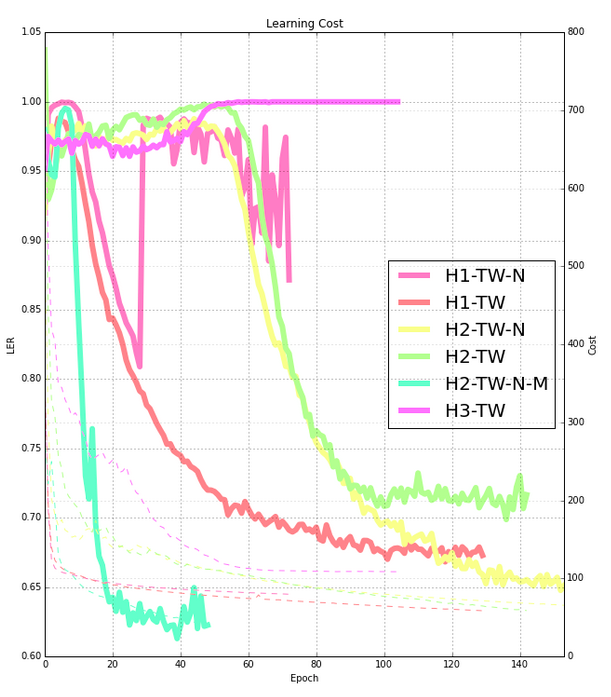
\includegraphics[width=9cm]{timeWindow_result_thin.png}
\caption{Training Result with different model under time-window, the prefix number of H represent the number of hidden layers, TW is the teime window, N and M abbreviate to Gaussian weight Noise and Momentum.  Color lines are corresponding to the left y-axis, the label error rate on validation data, dot lines are the CTC cost during training process, scale them on right y-axis.  The x-axis record down the epoch of each model,  we did not train the same epoch numbers for every model but stop them when the CTC cost start saturate. }
\end{figure}
\\
At the beginning of our training, we use MFCC feature with concatenation the previous three and following three at each frame for the larger input size.  Different model with and without the Gaussian noise.  According to the figure 1, system can't learn anything if the input layers is larger then 3, so we do not put the layer larger then 3 in our figure.  With only one hidden layer, model without noise seems better then the one with, however, this statement is not true with two hidden layer.  Out best result with time-window is the 2 hidden layer model with noise, momentum and clipping, the label error rate is 0.62.  Here we add clipping to prevent the too large or too small value when updating the parameter of our model[6] but we have not verify whether it should use with LSTM neurons.  \\
Later of our training, due to the lots of paper mentions that as well as the distorted data being used, time-window  approach suffer from the fact that the range of useful context is generally unknown.  Comparison between whether use the time-window propose in fig. 2.  Evidence indicate that there are not obviously progress or regress in our model.  For there's no progress in training, there's no reason to use the time-window as our input.  Last we try the bottleneck feature without time-window on our training.  At first we got a huge success on label error rate of validation data, then we try the deeper model which 3 and 4 hidden layers, but all of them can't learn anything ( the label error rate saturate around 1 ).  Finally we reduce the number of neurons in each hidden layer and it start learn from the data.  Three models we pick to do the experiment on test data, the H2-M-N model with LER is 0.62, the H2-M-BNF with LER is 0.44 and the H4(100)-M-BNF is  0.45.  Three results are 0.71, 0.68 and 0.66 which almost have no difference.  Additional beam-search is implement for test the word error rate (WER). Instead of combine language model, we try all 2000-best result to calculate WER, but still get nothing, so we stop our experiment on here.

\begin{figure}[h]
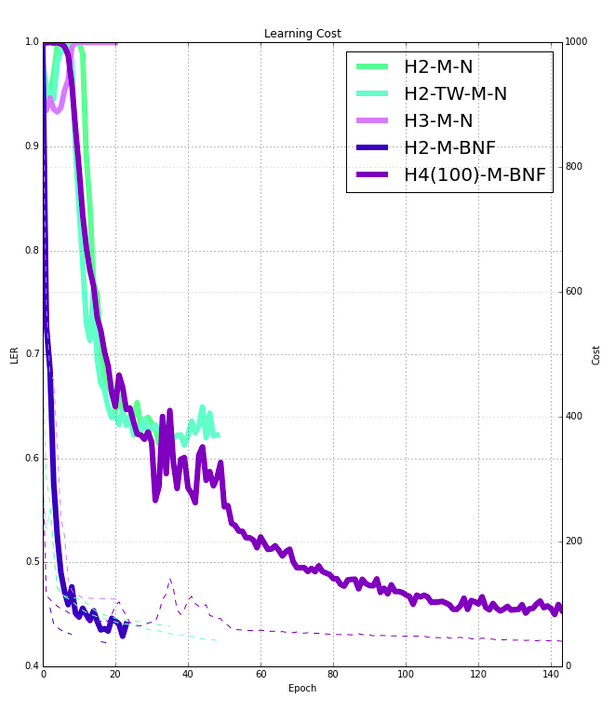
\includegraphics[width=9cm]{best_result_thin.png}
\caption{ Training Result without time-window, the TW, H, M, N is the same abbreviation as Fig. 1. New term BNF abbreviate to bottle-neck feature.  There's (100) behind the H4 to remind that each hidden layer in that model only get 100 neurons instead of 250.  Notice that the BNF model all train with Gaussian noise. }
\end{figure}


\section{Discuss and Conclusion}
According to our experiment result, there is no good enough label error rate for us to predict the word sequence and we stuck our score on testing data around 70\% even the bottleneck feature exhibit the better score on training data.  The first observation is that when we increase the number of total weight, the whole system become untrainable even with enough epoch, we attribute the untrainable evidence much to the less of training data.  Second, them seems a overfitting on the bottleneck feature, however, we had separate the speaker on validation set, so, there's no reason to perform the problem, the overfitting most probably due to the extracting process.  Although the experiment results is not indicate that the system is good enough to do a speech recognition test.  The provided character-level transcription on the low-resource language, the RNN-CTC system have being proof that it indeed learn something on the language.  The following examples is randomly picking decoding sentence in our Model. \\

The validation data with label error rate = 0.44 \\
\it{ Target:  o ngano diay muuban ka \\
Output:  o manga diay mobanka \\
Target:  ? ka didto sigi ra og tindog \\
Output:   h bai to giy ngtndog \\
Target:  ay usahay lang dili' man pod siya ingon nga dalo' piro \\
Output:  ay salang wa' po sa ingaon dalo piro3 \\}

The testing data with label error rate = 0.71\\
\it{ target: mga pila na kadto katuig wala' pa siya katrabaho mas nauna pa gani' siya og graduate gani'\\
output: mangatila napo katoli ula a sa katrba bassawu na sa  radde nadi\\
target: sa imo nga papa wala' diay ka na na\\ 
output: naimo ng pata wala diin ta nana\\
target: ? si lemon\\ 
output: idi\\ }

First glance at those data, obviously seem that almost all the sentence learn some pattern from the system.  Nonetheless we still discover some sentence that learn nothing at all.  On the testing result, we found that there are many sentence get the label error rate around 40\%, at the mean time, also mant sentence get ehe LER around 1.  Huge variance on LER but we have no good explanation except the not sufficient data.  For the experiment here, we depart the word meaning on Cebuano language, so we don't think the less word overlap affect our result.  In conclusion, result shows that even on under-resources language an end-to-end system is a good method to do the acoustic recognition task and we can keep going study how fix the system to get the better result.  

% use section* for acknowledgment
\section*{Acknowledgment}
Special thanks to our professor Hung-Yi Lee, who open a course named {\it Machine Learning and having it deep and structured (2015,Spring)} in National Taiwan University, all of my knowledge about neural network are learning from the class and project also inspired by the final project in that course which is build an ASR system on English. 

% references section
\begin{thebibliography}{1}

%1.
\bibitem{Basecier} L. Besacier, {\it Automatic Speech Recognition for Under-Resourced Languages: A Survey}

%2
\bibitem{Grave} A. Grave, {\it Towards End-to-End Speech Recognition
with Recurrent Neural Networks}

%3
\bibitem{Grave} A. Grave, {\it Connectionist Temporal Classification: Labelling Unsegmented Sequence Data with Recurrent Neural Network}

%4
\bibitem{Grave} A. Grace, {\it Supervised Sequence Labelling with Recurrent Neural Network}

%5
\bibitem{Hocheriter} S. Hochreiter, {\it Long Short-term memory}

%6
\bibitem{Pascanu} R. Pascanu , {\it On the difficulty of training recurrent neural networks}

%7
\bibitem{Schuster} M. Schuster , {\it Bidirectional Recurrent Neural Networks}

%8
\bibitem{Grave} A. Grace, {\it Bidirectional LSTM Networks for Improved Phoneme Classification and Recognition}

%9
\bibitem{Grezl} F. Grezl, {\it Probabilistic and Bottle-Neck Feature for LVCSR of Meetings}

%10
\bibitem{Tomas} S. Tomas, {\it Deep Neural Network Features and Semi-supervised Training For Low Resource Speech Recognition}

%11
\bibitem{Jim} Jim, {\it An Analysis of Noise in Recurrent Neural Networks Convergence and Generalization}

%12
\bibitem{Lasagne} Lasagne, craffel/nntools, {\it https://github.com/craffel/nntools}

%13
\bibitem{CTC} mohammadpz/CTC-Connectionist-Temporal-Classification, {\it https://github.com/mohammadpz/CTC-Connectionist-Temporal-Classification/tree/no$\_$underflow }

\end{thebibliography}

\end{document}